\chapter{A Two-dimensional Transient Conduction Problem}
The four materials problem is a two-dimensional transient conduction problem. It consists in a long rod composed of four different materials with different properties. The general scheme of the problem is represented in figure \ref{fourmaterials}, and the dimensions of the materials, their properties, and the boundary conditions are in the tables below.
\begin{figure}[h]
	\centering
	\includegraphics[scale = 0.6]{FourMaterials/Fourmaterials}
	\caption{General scheme of the four materials problem}
	\label{fourmaterials}
\end{figure}
\begin{table}[h!]
	\centering
	\begin{tabular}{ |c|c|c|}
		\hline
		  & x [m] & y [m] \\ \hline
		 $p_{1}$ & $0.50$ & $0.40$ \\ \hline
		 $p_{2}$ & $0.50$ & $0.70$ \\ \hline
		 $p_{3}$ & $1.10$ & $0.80$ \\ \hline
	\end{tabular}
\caption{Problem coordinates}
\end{table}
\begin{table}[h!]
	\centering
	\begin{tabular}{ |c|c|c|c| }
		\hline
		& $\rho [kg/m^{3}]$ & $c_{P} [J/kgK]$ & $\lambda [W/mK]$ \\ \hline
		$M_{1}$ & $1500.00$ & $750.00$ & $170.00$ \\ \hline
		$M_{2}$ & $1600.00$ & $770.00$ & $140.00$ \\ \hline
		$M_{3}$ & $1900.00$ & $810.00$ & $200.00$ \\ \hline
		$M_{4}$ & $2500.00$ & $930.00$ & $140.00$ \\ \hline
	\end{tabular}
\caption{Physical properties of the materials}
\end{table}
\begin{table}
	\centering
	\begin{tabular}{ |c|c|}
		\hline
		Cavity wall & Boundary condition \\ \hline
		Bottom & Isotherm at $T=23.00 ^{\circ}C$ \\ \hline
		Top & Uniform $Q_{flow}=60.00 W/m$ length \\ \hline
		Left & In contact with a fluid at $T_{g}=33.00 ^{\circ}C$ and heat transfer coefficient $9.00 W/m^{2}K$ \\ \hline
		Right & Uniform temperature $T=8.00+0.005t ^{\circ}C$ (where $t$ is the time in seconds) \\ \hline
	\end{tabular}
\caption{Boundary conditions}
\end{table}

The initial temperature field is $T=8.00 ^{\circ}C$.

\section{Discretization}
The spatial discretization of the problem is that described in section \ref{SpatialDiscretizationConduction}. However, since there are different materials, each of them is discretized separately. The variable $M_{1}$ is the number of control volumes in the vertical direction from $Y=0$ to the point $p_{1}$, $M_{2}$ from $p_{1}$ to $p_{2}$ and $M_{3}$ form $p_{2}$ to $p_{3}$. In the horizontal direction, the variable $N_{1}$ is the number of control volumes from $X=0$ to the point $p_{1}$ and $N_{2}$ from $p_{1}$ to $p_{3}$.
\begin{table}[h]
	\centering
	\begin{tabular}{ |c|c|c|c|c|c| }
		\hline
		$M_{1}$ & $M_{2}$ & $M_{3}$ & $N_{1}$ & $N_{2}$ & $\delta$ \\ \hline
		$40$ & $30$ & $10$ & $50$ & $60$ & $10^{-3}$ \\ \hline
	\end{tabular}
	\caption{Numerical parameters of the four materials problem}
\end{table}

\section{Boundary conditions}
The coefficients of the discretized equation in the inner nodes are the ones of the section \ref{DiscrCond}. The outer walls of the rod have special conditions, so each of them has to be studied in order to determine which coefficients of their boundary nodes are different.

In the left wall, there is convection with the fluid outside of the road. In order to fulfil this condition, some coefficients have to be recalculated:
\begin{equation}
a_{W}=0
\end{equation}
\begin{equation}
a_{P}=a_{E}+a_{W}+a_{N}+a_{S}+\frac{\rho_{P}V_{P}\bar{c}_{P}}{\Delta t}+\frac{\beta}{\frac{1}{\alpha}+\frac{d_{Pw}}{\lambda_{P}}}
\end{equation}
\begin{multline}
b_{P}=\frac{\rho_{P}V_{P}\bar{c}_{P}T_{P}^{n}}{\Delta t}+\beta\left(\dot{q}_{vP}^{n+1}V_{P}+\frac{T_{g}}{\frac{1}{\alpha}+\frac{d_{Pw}}{\lambda_{P}}}\right) \\
+\left(1-\beta\right)\left[\frac{T_{g}-T_{P}}{\frac{1}{\alpha}+\frac{d_{Pw}}{\lambda_{P}}}+\lambda_{e}\frac{T_{E}-T_{P}}{d_{PE}}S_{e}-\lambda_{s}\frac{T_{P}-T_{S}}{d_{PS}}S_{s}+\lambda_{n}\frac{T_{N}-T_{P}}{d_{PN}}S_{n}+\dot{q}_{vP}V_{P}\right]^{n}
\end{multline}

There is a constant heat flux in the top wall. The value of this flux is given for the total wall, so it is assumed that it is uniformly distributed over the top wall. In this case, the coefficients that change their value are:
\begin{equation}
a_{N}=0
\end{equation}
\begin{multline}
b_{P}=\frac{\rho_{P}V_{P}\bar{c}_{P}T_{P}^{n}}{\Delta t}+\beta\dot{q}_{vP}^{n+1}V_{P}+Q_{flow}\frac{S_{n}}{S_{top}} \\
+\left(1-\beta\right)\left[-\lambda_{w}\frac{T_{P}-T_{W}}{d_{PW}}S_{w}+\lambda_{e}\frac{T_{E}-T_{P}}{d_{PE}}S_{e}-\lambda_{s}\frac{T_{P}-T_{S}}{d_{PS}}S_{s}+\dot{q}_{vP}V_{P}\right]^{n}
\end{multline}

In the right wall, the temperature $T_{r}$ is given, and it changes over time. The coefficients are very similar to those of the general case. The only differences are:
\begin{equation}
a_{E}=0
\end{equation}
\begin{equation}
a_P=a_{E}+a_{W}+a_{N}+a_{S}+\frac{\rho_{P}V_{P}\bar{c}_{P}}{\Delta t}+\beta\frac{\lambda_{P}S_{e}}{d_{Pe}}
\end{equation}
\begin{multline}
b_{P}=\frac{\rho_{P}V_{P}\bar{c}_{P}T_{P}^{n}}{\Delta t}+\beta\left(\dot{q}_{vP}^{n+1}V_{P}+\frac{\lambda_{P}S_{e}}{d_{Pe}}T_{r}^{n+1}\right) \\
+\left(1-\beta\right)\left[-\lambda_{w}\frac{T_{P}-T_{W}}{d_{PW}}S_{w}+\lambda_{P}\frac{T_{r}-T_{P}}{d_{Pe}}S_{e}-\lambda_{s}\frac{T_{P}-T_{S}}{d_{PS}}S_{s}+\lambda_{n}\frac{T_{N}-T_{P}}{d_{PN}}S_{n}+\dot{q}_{vP}V_{P}\right]^{n}
\end{multline}

Finally, in the bottom wall, the temperature $T_{b}$ is also given, but it is constant over time. The approach is very similar to that of the right wall, so that the different coefficients are:
\begin{equation}
a_{S}=0
\end{equation}
\begin{equation}
a_P=a_{E}+a_{W}+a_{N}+a_{S}+\frac{\rho_{P}V_{P}\bar{c}_{P}}{\Delta t}+\beta\frac{\lambda_{P}S_{s}}{d_{Ps}}
\end{equation}
\begin{multline}
b_{P}=\frac{\rho_{P}V_{P}\bar{c}_{P}T_{P}^{n}}{\Delta t}+\beta\left(\dot{q}_{vP}^{n+1}V_{P}+\frac{\lambda_{P}S_{s}}{d_{Ps}}T_{b}\right) \\
+\left(1-\beta\right)\left[-\lambda_{w}\frac{T_{P}-T_{W}}{d_{PW}}S_{w}+\lambda_{e}\frac{T_{E}-T_{P}}{d_{PE}}S_{e}-\lambda_{P}\frac{T_{P}-T_{b}}{d_{Ps}}S_{s}+\lambda_{n}\frac{T_{N}-T_{P}}{d_{PN}}S_{n}+\dot{q}_{vP}V_{P}\right]^{n}
\end{multline}

\section{Algorithm}
The algorithm used in this convection problem is represented below. In this case, some of the discretization coefficients are constant, but sometimes they are not. These would change slightly the algorithm used.
\begin{figure}[h!]
	\centering
	\includegraphics[scale=0.154]{FourMaterials/algorithm}
\end{figure}

\section{Results}
To verify the simulation, the results obtained are compared with some reference values for a time of 5000 s. As it can be seen in figures \ref{ref4M} and \ref{ref4M}, the results of the code are very similar to the reference values.
\begin{figure}[h!]
	\centering
	\includegraphics[scale=0.55]{FourMaterials/reference}
	\caption{Reference value: Instantaneous isotherms at $t=10000/2$ s}
	\label{ref4M}
\end{figure}
\begin{figure}[h!]
	\centering
	\input{FourMaterials/Resultats5000}
	\caption{Instantaneous isotherm at t=5000 s}
	\label{plot4M}
\end{figure}

The four materials problem is transitory. Since the temperature in the right wall changes over time, it never reaches a steady state. To obtain some results, the final time of the simulation has been chosen to be 10000 s, as in the results of the figure \ref{4Mfinal}.
\begin{figure}[h]
	\centering
	% GNUPLOT: LaTeX picture with Postscript
\begingroup
  \makeatletter
  \providecommand\color[2][]{%
    \GenericError{(gnuplot) \space\space\space\@spaces}{%
      Package color not loaded in conjunction with
      terminal option `colourtext'%
    }{See the gnuplot documentation for explanation.%
    }{Either use 'blacktext' in gnuplot or load the package
      color.sty in LaTeX.}%
    \renewcommand\color[2][]{}%
  }%
  \providecommand\includegraphics[2][]{%
    \GenericError{(gnuplot) \space\space\space\@spaces}{%
      Package graphicx or graphics not loaded%
    }{See the gnuplot documentation for explanation.%
    }{The gnuplot epslatex terminal needs graphicx.sty or graphics.sty.}%
    \renewcommand\includegraphics[2][]{}%
  }%
  \providecommand\rotatebox[2]{#2}%
  \@ifundefined{ifGPcolor}{%
    \newif\ifGPcolor
    \GPcolortrue
  }{}%
  \@ifundefined{ifGPblacktext}{%
    \newif\ifGPblacktext
    \GPblacktexttrue
  }{}%
  % define a \g@addto@macro without @ in the name:
  \let\gplgaddtomacro\g@addto@macro
  % define empty templates for all commands taking text:
  \gdef\gplbacktext{}%
  \gdef\gplfronttext{}%
  \makeatother
  \ifGPblacktext
    % no textcolor at all
    \def\colorrgb#1{}%
    \def\colorgray#1{}%
  \else
    % gray or color?
    \ifGPcolor
      \def\colorrgb#1{\color[rgb]{#1}}%
      \def\colorgray#1{\color[gray]{#1}}%
      \expandafter\def\csname LTw\endcsname{\color{white}}%
      \expandafter\def\csname LTb\endcsname{\color{black}}%
      \expandafter\def\csname LTa\endcsname{\color{black}}%
      \expandafter\def\csname LT0\endcsname{\color[rgb]{1,0,0}}%
      \expandafter\def\csname LT1\endcsname{\color[rgb]{0,1,0}}%
      \expandafter\def\csname LT2\endcsname{\color[rgb]{0,0,1}}%
      \expandafter\def\csname LT3\endcsname{\color[rgb]{1,0,1}}%
      \expandafter\def\csname LT4\endcsname{\color[rgb]{0,1,1}}%
      \expandafter\def\csname LT5\endcsname{\color[rgb]{1,1,0}}%
      \expandafter\def\csname LT6\endcsname{\color[rgb]{0,0,0}}%
      \expandafter\def\csname LT7\endcsname{\color[rgb]{1,0.3,0}}%
      \expandafter\def\csname LT8\endcsname{\color[rgb]{0.5,0.5,0.5}}%
    \else
      % gray
      \def\colorrgb#1{\color{black}}%
      \def\colorgray#1{\color[gray]{#1}}%
      \expandafter\def\csname LTw\endcsname{\color{white}}%
      \expandafter\def\csname LTb\endcsname{\color{black}}%
      \expandafter\def\csname LTa\endcsname{\color{black}}%
      \expandafter\def\csname LT0\endcsname{\color{black}}%
      \expandafter\def\csname LT1\endcsname{\color{black}}%
      \expandafter\def\csname LT2\endcsname{\color{black}}%
      \expandafter\def\csname LT3\endcsname{\color{black}}%
      \expandafter\def\csname LT4\endcsname{\color{black}}%
      \expandafter\def\csname LT5\endcsname{\color{black}}%
      \expandafter\def\csname LT6\endcsname{\color{black}}%
      \expandafter\def\csname LT7\endcsname{\color{black}}%
      \expandafter\def\csname LT8\endcsname{\color{black}}%
    \fi
  \fi
    \setlength{\unitlength}{0.0500bp}%
    \ifx\gptboxheight\undefined%
      \newlength{\gptboxheight}%
      \newlength{\gptboxwidth}%
      \newsavebox{\gptboxtext}%
    \fi%
    \setlength{\fboxrule}{0.5pt}%
    \setlength{\fboxsep}{1pt}%
\begin{picture}(7200.00,5040.00)%
    \gplgaddtomacro\gplbacktext{%
    }%
    \gplgaddtomacro\gplfronttext{%
      \put(936,624){\makebox(0,0){\strut{}$0$}}%
      \put(1905,624){\makebox(0,0){\strut{}$0.2$}}%
      \put(2874,624){\makebox(0,0){\strut{}$0.4$}}%
      \put(3842,624){\makebox(0,0){\strut{}$0.6$}}%
      \put(4811,624){\makebox(0,0){\strut{}$0.8$}}%
      \put(5780,624){\makebox(0,0){\strut{}$1$}}%
      \put(748,938){\makebox(0,0)[r]{\strut{}$0$}}%
      \put(748,1361){\makebox(0,0)[r]{\strut{}$0.1$}}%
      \put(748,1784){\makebox(0,0)[r]{\strut{}$0.2$}}%
      \put(748,2207){\makebox(0,0)[r]{\strut{}$0.3$}}%
      \put(748,2630){\makebox(0,0)[r]{\strut{}$0.4$}}%
      \put(748,3053){\makebox(0,0)[r]{\strut{}$0.5$}}%
      \put(748,3476){\makebox(0,0)[r]{\strut{}$0.6$}}%
      \put(748,3899){\makebox(0,0)[r]{\strut{}$0.7$}}%
      \put(748,4322){\makebox(0,0)[r]{\strut{}$0.8$}}%
      \put(6796,938){\makebox(0,0)[l]{\strut{}$20$}}%
      \put(6796,1361){\makebox(0,0)[l]{\strut{}$25$}}%
      \put(6796,1784){\makebox(0,0)[l]{\strut{}$30$}}%
      \put(6796,2207){\makebox(0,0)[l]{\strut{}$35$}}%
      \put(6796,2630){\makebox(0,0)[l]{\strut{}$40$}}%
      \put(6796,3053){\makebox(0,0)[l]{\strut{}$45$}}%
      \put(6796,3476){\makebox(0,0)[l]{\strut{}$50$}}%
      \put(6796,3899){\makebox(0,0)[l]{\strut{}$55$}}%
      \put(6796,4322){\makebox(0,0)[l]{\strut{}$60$}}%
    }%
    \gplbacktext
    \put(0,0){\includegraphics{FourMaterials/Resultats}}%
    \gplfronttext
  \end{picture}%
\endgroup

	\caption{Instantaneous plot at t=10000 s}
	\label{4Mfinal}
\end{figure}

Nevertheless, to analyse the results obtained, the same simulation has been run for a homogeneous material (figure \ref{HomoM2}). The geometrical parameters and the boundary conditions have been maintained, but the physical properties of the whole material are those of the section $M_{2}$ of the four materials problem.
\begin{figure}[h]
	\centering
	% GNUPLOT: LaTeX picture with Postscript
\begingroup
  \makeatletter
  \providecommand\color[2][]{%
    \GenericError{(gnuplot) \space\space\space\@spaces}{%
      Package color not loaded in conjunction with
      terminal option `colourtext'%
    }{See the gnuplot documentation for explanation.%
    }{Either use 'blacktext' in gnuplot or load the package
      color.sty in LaTeX.}%
    \renewcommand\color[2][]{}%
  }%
  \providecommand\includegraphics[2][]{%
    \GenericError{(gnuplot) \space\space\space\@spaces}{%
      Package graphicx or graphics not loaded%
    }{See the gnuplot documentation for explanation.%
    }{The gnuplot epslatex terminal needs graphicx.sty or graphics.sty.}%
    \renewcommand\includegraphics[2][]{}%
  }%
  \providecommand\rotatebox[2]{#2}%
  \@ifundefined{ifGPcolor}{%
    \newif\ifGPcolor
    \GPcolortrue
  }{}%
  \@ifundefined{ifGPblacktext}{%
    \newif\ifGPblacktext
    \GPblacktexttrue
  }{}%
  % define a \g@addto@macro without @ in the name:
  \let\gplgaddtomacro\g@addto@macro
  % define empty templates for all commands taking text:
  \gdef\gplbacktext{}%
  \gdef\gplfronttext{}%
  \makeatother
  \ifGPblacktext
    % no textcolor at all
    \def\colorrgb#1{}%
    \def\colorgray#1{}%
  \else
    % gray or color?
    \ifGPcolor
      \def\colorrgb#1{\color[rgb]{#1}}%
      \def\colorgray#1{\color[gray]{#1}}%
      \expandafter\def\csname LTw\endcsname{\color{white}}%
      \expandafter\def\csname LTb\endcsname{\color{black}}%
      \expandafter\def\csname LTa\endcsname{\color{black}}%
      \expandafter\def\csname LT0\endcsname{\color[rgb]{1,0,0}}%
      \expandafter\def\csname LT1\endcsname{\color[rgb]{0,1,0}}%
      \expandafter\def\csname LT2\endcsname{\color[rgb]{0,0,1}}%
      \expandafter\def\csname LT3\endcsname{\color[rgb]{1,0,1}}%
      \expandafter\def\csname LT4\endcsname{\color[rgb]{0,1,1}}%
      \expandafter\def\csname LT5\endcsname{\color[rgb]{1,1,0}}%
      \expandafter\def\csname LT6\endcsname{\color[rgb]{0,0,0}}%
      \expandafter\def\csname LT7\endcsname{\color[rgb]{1,0.3,0}}%
      \expandafter\def\csname LT8\endcsname{\color[rgb]{0.5,0.5,0.5}}%
    \else
      % gray
      \def\colorrgb#1{\color{black}}%
      \def\colorgray#1{\color[gray]{#1}}%
      \expandafter\def\csname LTw\endcsname{\color{white}}%
      \expandafter\def\csname LTb\endcsname{\color{black}}%
      \expandafter\def\csname LTa\endcsname{\color{black}}%
      \expandafter\def\csname LT0\endcsname{\color{black}}%
      \expandafter\def\csname LT1\endcsname{\color{black}}%
      \expandafter\def\csname LT2\endcsname{\color{black}}%
      \expandafter\def\csname LT3\endcsname{\color{black}}%
      \expandafter\def\csname LT4\endcsname{\color{black}}%
      \expandafter\def\csname LT5\endcsname{\color{black}}%
      \expandafter\def\csname LT6\endcsname{\color{black}}%
      \expandafter\def\csname LT7\endcsname{\color{black}}%
      \expandafter\def\csname LT8\endcsname{\color{black}}%
    \fi
  \fi
    \setlength{\unitlength}{0.0500bp}%
    \ifx\gptboxheight\undefined%
      \newlength{\gptboxheight}%
      \newlength{\gptboxwidth}%
      \newsavebox{\gptboxtext}%
    \fi%
    \setlength{\fboxrule}{0.5pt}%
    \setlength{\fboxsep}{1pt}%
\begin{picture}(7200.00,5040.00)%
    \gplgaddtomacro\gplbacktext{%
    }%
    \gplgaddtomacro\gplfronttext{%
      \put(1273,624){\makebox(0,0){\strut{}$0$}}%
      \put(2119,624){\makebox(0,0){\strut{}$0.2$}}%
      \put(2966,624){\makebox(0,0){\strut{}$0.4$}}%
      \put(3811,624){\makebox(0,0){\strut{}$0.6$}}%
      \put(4658,624){\makebox(0,0){\strut{}$0.8$}}%
      \put(5504,624){\makebox(0,0){\strut{}$1$}}%
      \put(1085,938){\makebox(0,0)[r]{\strut{}$0$}}%
      \put(1085,1361){\makebox(0,0)[r]{\strut{}$0.1$}}%
      \put(1085,1784){\makebox(0,0)[r]{\strut{}$0.2$}}%
      \put(1085,2207){\makebox(0,0)[r]{\strut{}$0.3$}}%
      \put(1085,2630){\makebox(0,0)[r]{\strut{}$0.4$}}%
      \put(1085,3053){\makebox(0,0)[r]{\strut{}$0.5$}}%
      \put(1085,3476){\makebox(0,0)[r]{\strut{}$0.6$}}%
      \put(1085,3899){\makebox(0,0)[r]{\strut{}$0.7$}}%
      \put(1085,4322){\makebox(0,0)[r]{\strut{}$0.8$}}%
      \put(6408,938){\makebox(0,0)[l]{\strut{}$15$}}%
      \put(6408,1314){\makebox(0,0)[l]{\strut{}$20$}}%
      \put(6408,1690){\makebox(0,0)[l]{\strut{}$25$}}%
      \put(6408,2066){\makebox(0,0)[l]{\strut{}$30$}}%
      \put(6408,2442){\makebox(0,0)[l]{\strut{}$35$}}%
      \put(6408,2818){\makebox(0,0)[l]{\strut{}$40$}}%
      \put(6408,3194){\makebox(0,0)[l]{\strut{}$45$}}%
      \put(6408,3570){\makebox(0,0)[l]{\strut{}$50$}}%
      \put(6408,3946){\makebox(0,0)[l]{\strut{}$55$}}%
      \put(6408,4322){\makebox(0,0)[l]{\strut{}$60$}}%
    }%
    \gplbacktext
    \put(0,0){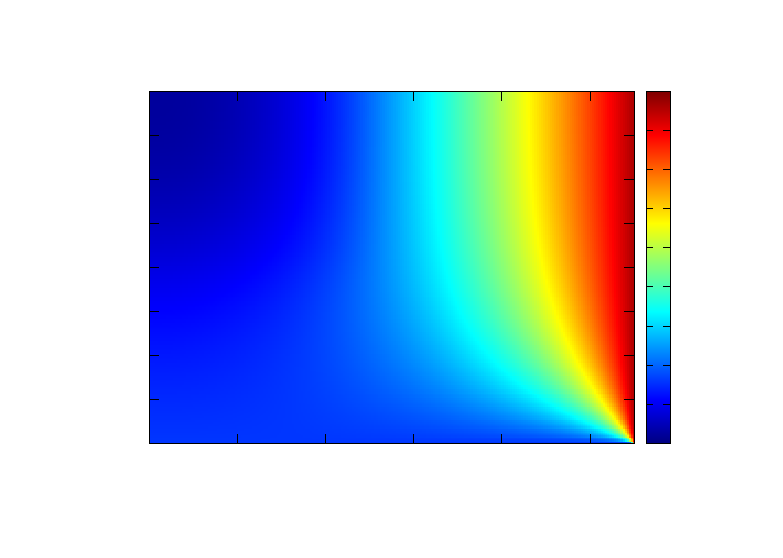
\includegraphics{FourMaterials/HomoM2}}%
    \gplfronttext
  \end{picture}%
\endgroup

	\caption{Instantaneous plot at t=10000 s for a homogeneous material}
	\label{HomoM2}
\end{figure}

Comparing both graphs, it can be stated that the final result is very similar in both cases. The main visible difference is that in the four materials problem, the higher temperatures move further to the left. In the original problem, the upper right region is made of the material $M_{4}$, which has the same conductivity as the homogeneous material $M_{2}$, but a higher density and specific heat, making the first material more capable of conducting the heat.